\chapter{Results}
\label{ch:results}
The Kalman filter and controls algorithms discussed in this thesis were implemented in software on a PackBot and run in an open field with an uneven surface consisting of dirt, gravel and asphalt as seen in Figure \ref{fig:resultsTestArea}. This testing area is difficult for the robots to navigate because pitch, roll and elevation have significant changes and the loose dirt and gravel can cause the tracks to slip leading to erroneous encoder data.

\begin{figure}[ht!]
	\centering
	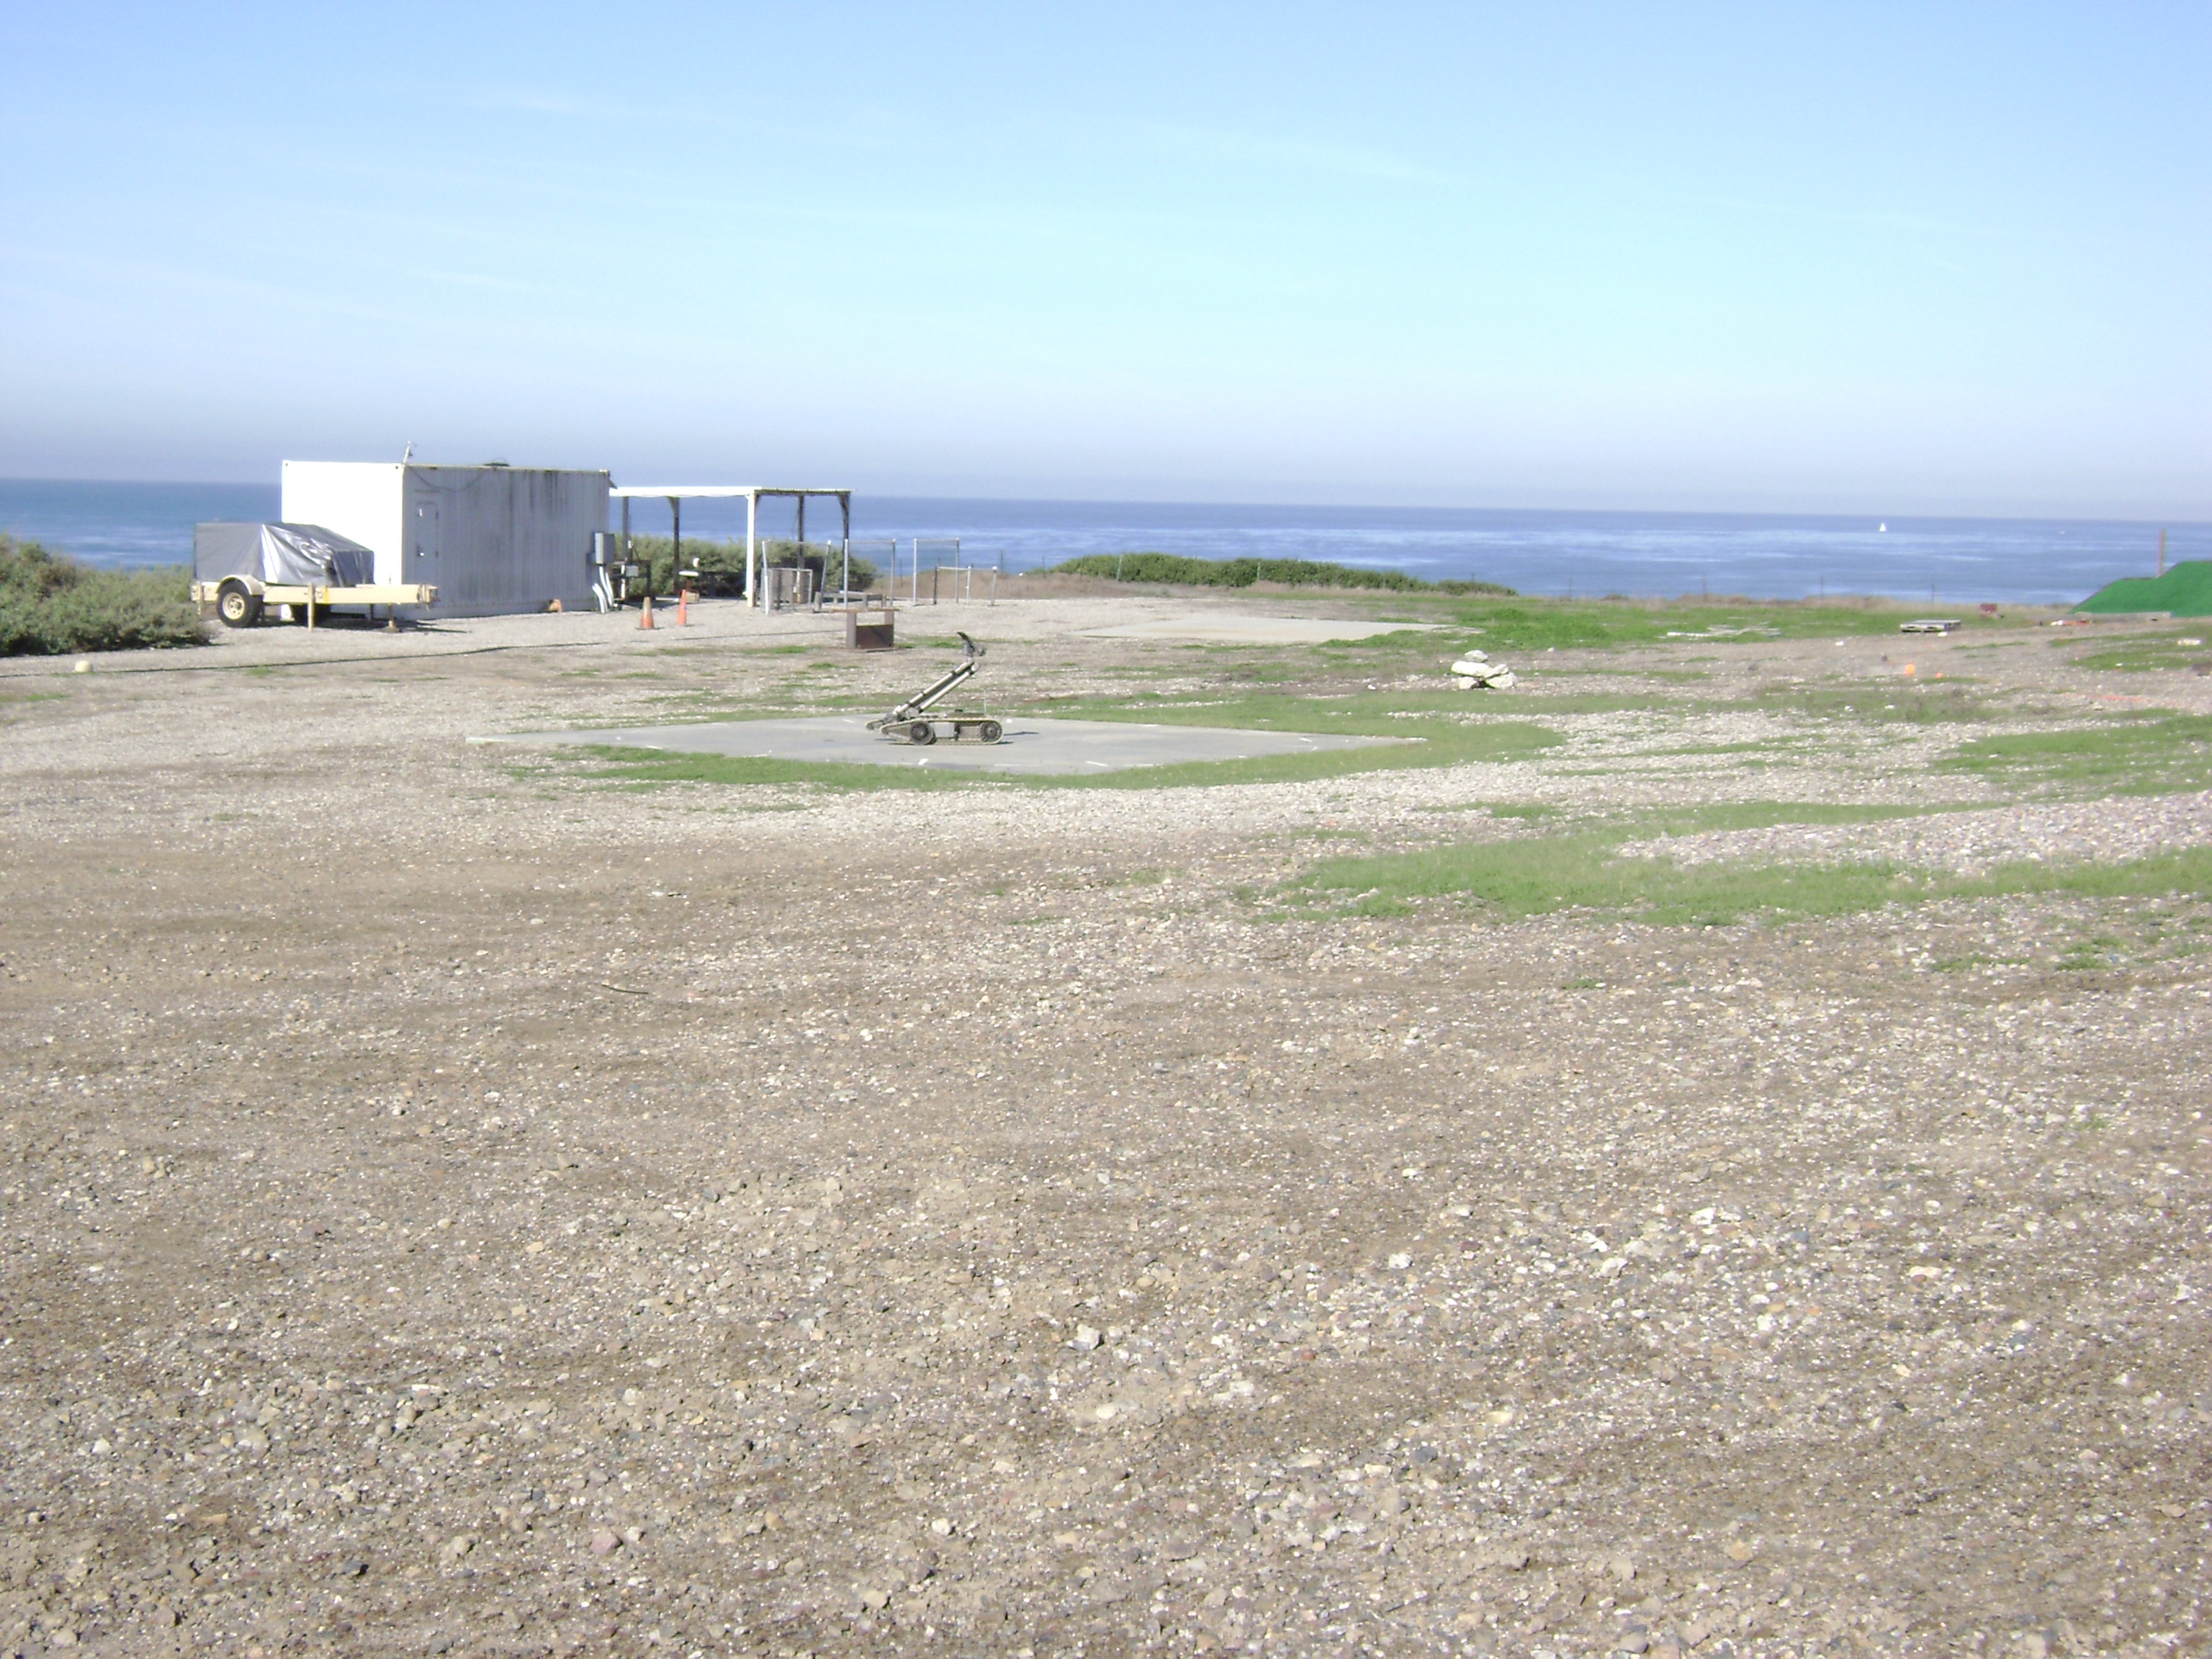
\includegraphics[width=.75\textwidth]{images/flightFieldTestArea}
	\caption{Robot Test Area}
	\label{fig:resultsTestArea}
\end{figure}

*** Run the robot again while varying the stages of improvements and put the results in Table \ref{tab:resultsKF}. ***
\begin{table}[ht!]
\caption{Kalman Filter Performance}
\small
\centering
\begin{tabular}{@{}llr@{}} \toprule
Stage       & RMS Error (m)  & Return Error (\%) \\ \midrule
Baseline    & 0              & 0                 \\
Fix KF Bugs & 0              & 0                 \\
Training    & 0              & 0                 \\ \bottomrule
\end{tabular}
\label{tab:resultsKF}
\end{table}

\section{Kalman Filter Results}
\label{sec:kfResults}
Model based with original noise models.

\begin{figure}[ht!]
	\centering
	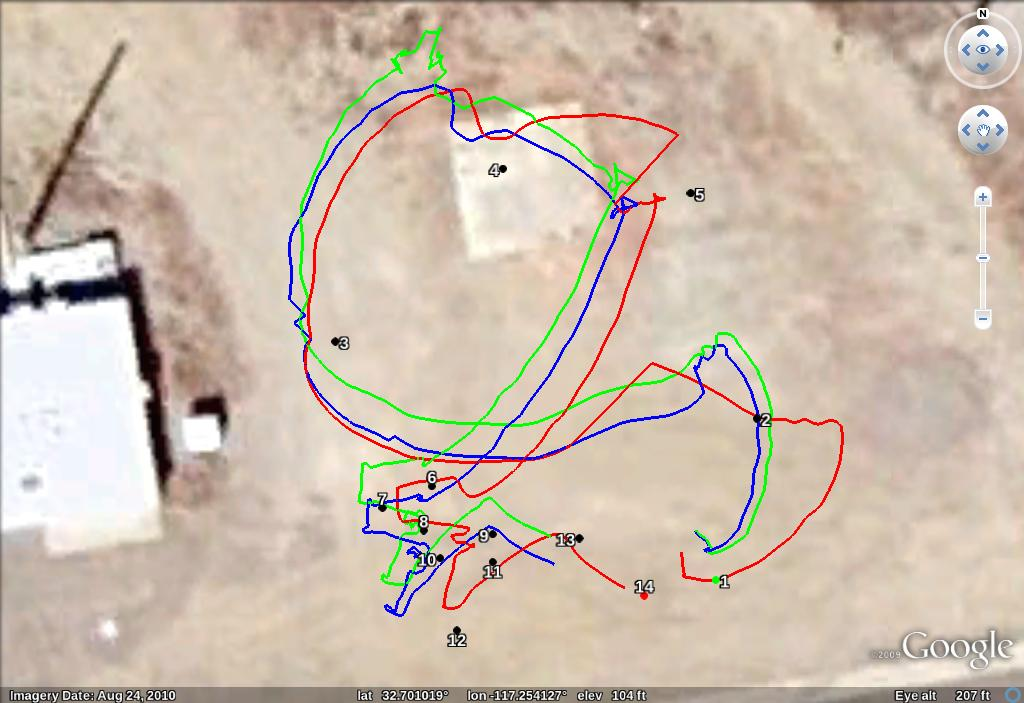
\includegraphics[width=.75\textwidth]{images/GE/20101203_1551_kf_lyapOrigQR}
	\caption{Model Based Controller with Original Noise Models}
	\label{fig:kfResults1}
\end{figure}

Model based with learned noise models.

\begin{figure}[ht!]
	\centering
	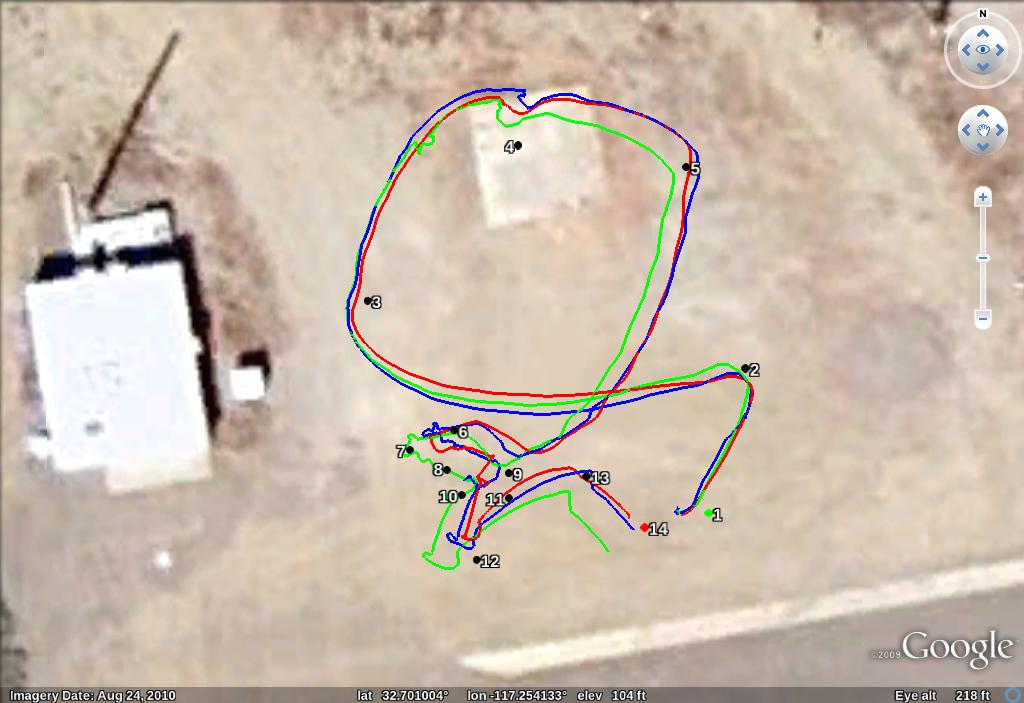
\includegraphics[width=.75\textwidth]{images/GE/20101203_1545_kf_lyapNewQR}
	\caption{Model Based Controller with Learned Noise Models}
	\label{fig:kfResults2}
\end{figure}

Model based with DGPS as input to Kalman filter and learned noise models.

\begin{figure}[ht!]
	\centering
	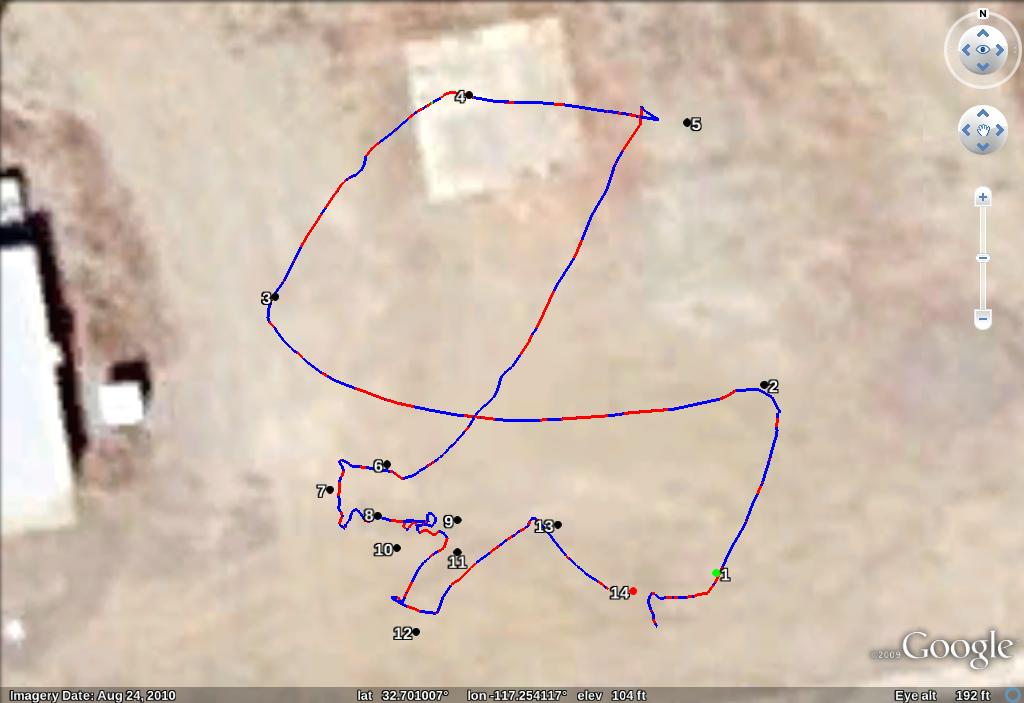
\includegraphics[width=.75\textwidth]{images/GE/20101203_1606_kf_lyapUsingDgpsNewQR}
	\caption{Model Based Controller with DGPS and Learned Noise Models}
	\label{fig:kfResults3}
\end{figure}

PID with original noise models.

\begin{figure}[ht!]
	\centering
	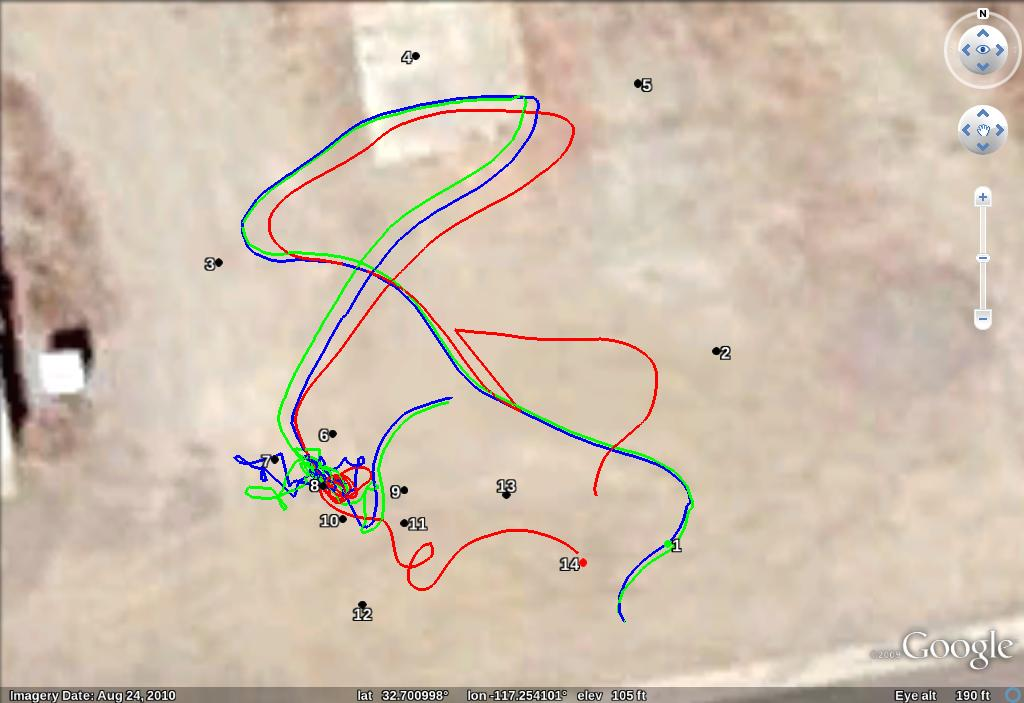
\includegraphics[width=.75\textwidth]{images/GE/20101203_1755_kf_pidOrigQR}
	\caption{PID Controller with Original Noise Models}
	\label{fig:kfResults4}
\end{figure}

PID with learned noise models.

\begin{figure}[ht!]
	\centering
	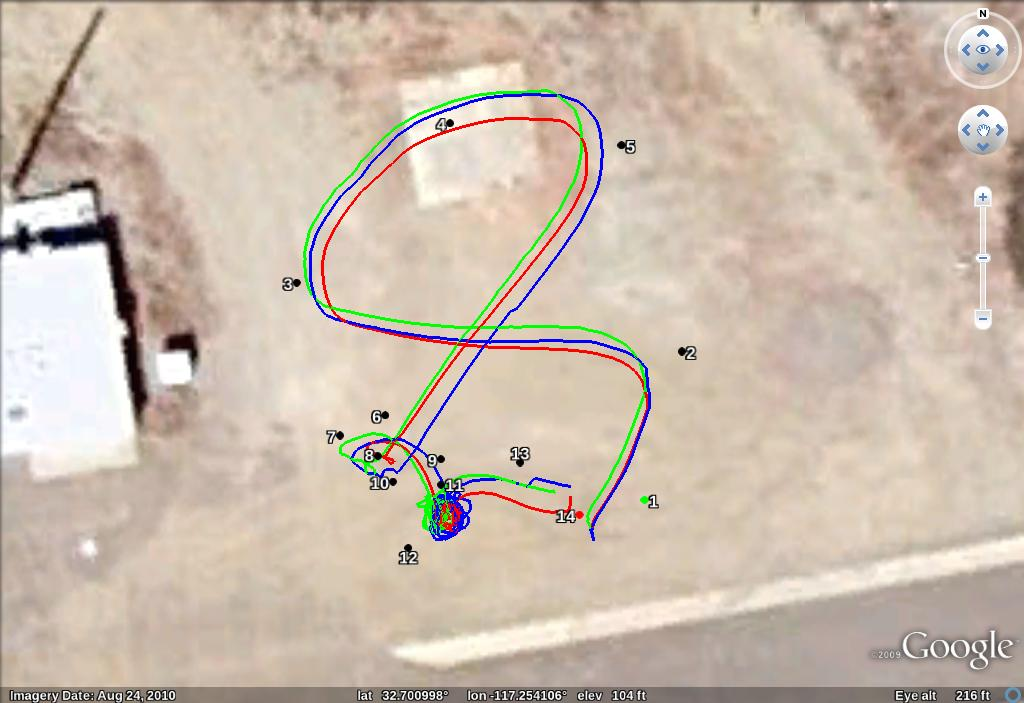
\includegraphics[width=.75\textwidth]{images/GE/20101203_1751_kf_pidNewQR}
	\caption{PID Controller with Learned Noise Models}
	\label{fig:kfResults5}
\end{figure}

PID with DGPS as input to Kalman filter and learned noise models.

\begin{figure}[ht!]
	\centering
	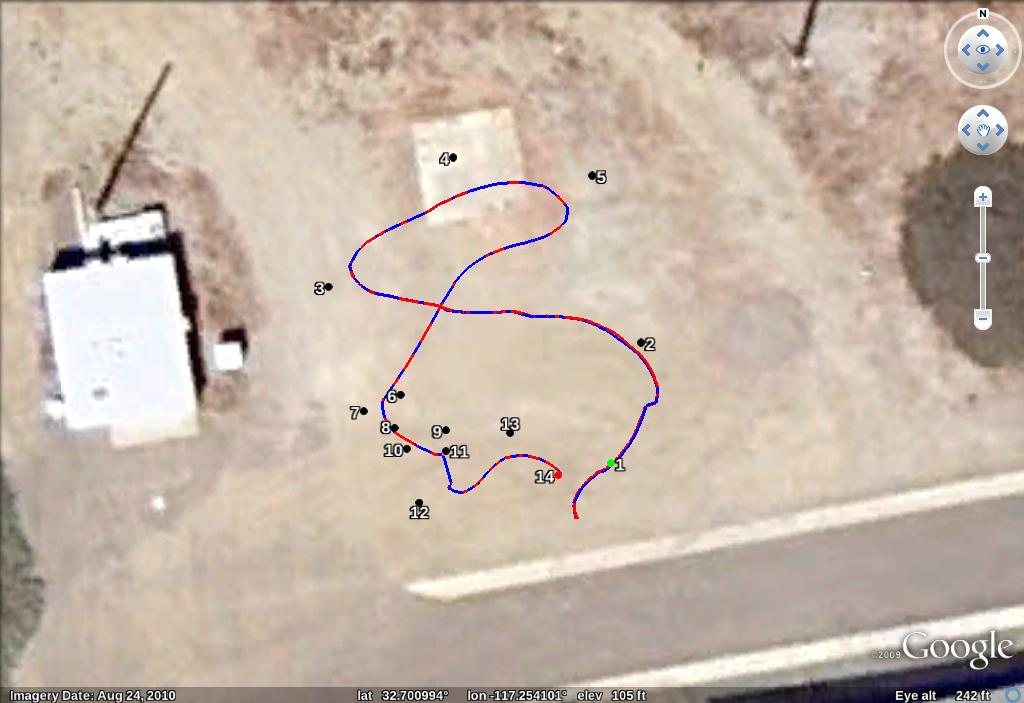
\includegraphics[width=.75\textwidth]{images/GE/20101203_1803_kf_pidUsingDgpsNewQR}
	\caption{PID Controller with DGPS and Learned Noise Models}
	\label{fig:kfResults6}
\end{figure}

\section{Model Based Controller Results}
\label{sec:lyapunovResults}
The control law derived in (\ref{eq:lyapunovControlLaw}) was tested in the previously described area in two different ways. The first set of results used a single set of gains and had the goal heading set to use the current heading of the robot so that $\theta^\star=\alpha$ as discussed in Chapter \ref{sec:lyapunovVariables}. Figure *** shows the actual position of the robot during navigation as well as the waypoints that defined the desired route.

Figures \ref{fig:resultsLyapunov1} - \ref{fig:resultsLyapunov6} shows how the linear and angular velocities changed over time as measured by the Kalman filter output. The gains used were $h=0.1$, $k=0.25$ and $\gamma=0.23$. A clear deceleration can be seen as the robot approaches each waypoint although the linear velocity does not go to zero until the final waypoint due to the use of the carrot in the path planner as discussed in Chapter \ref{sec:lyapunovVariables} for determing the error distance $e$. One of the consequences of using a model based controller is that a negative linear velocity was used after reaching the second waypoint and having the error angle $\alpha$ move towards the third waypoint which is rarely, if ever, encountered when using the original PID controller.

\begin{figure}[ht!]
	\centering
	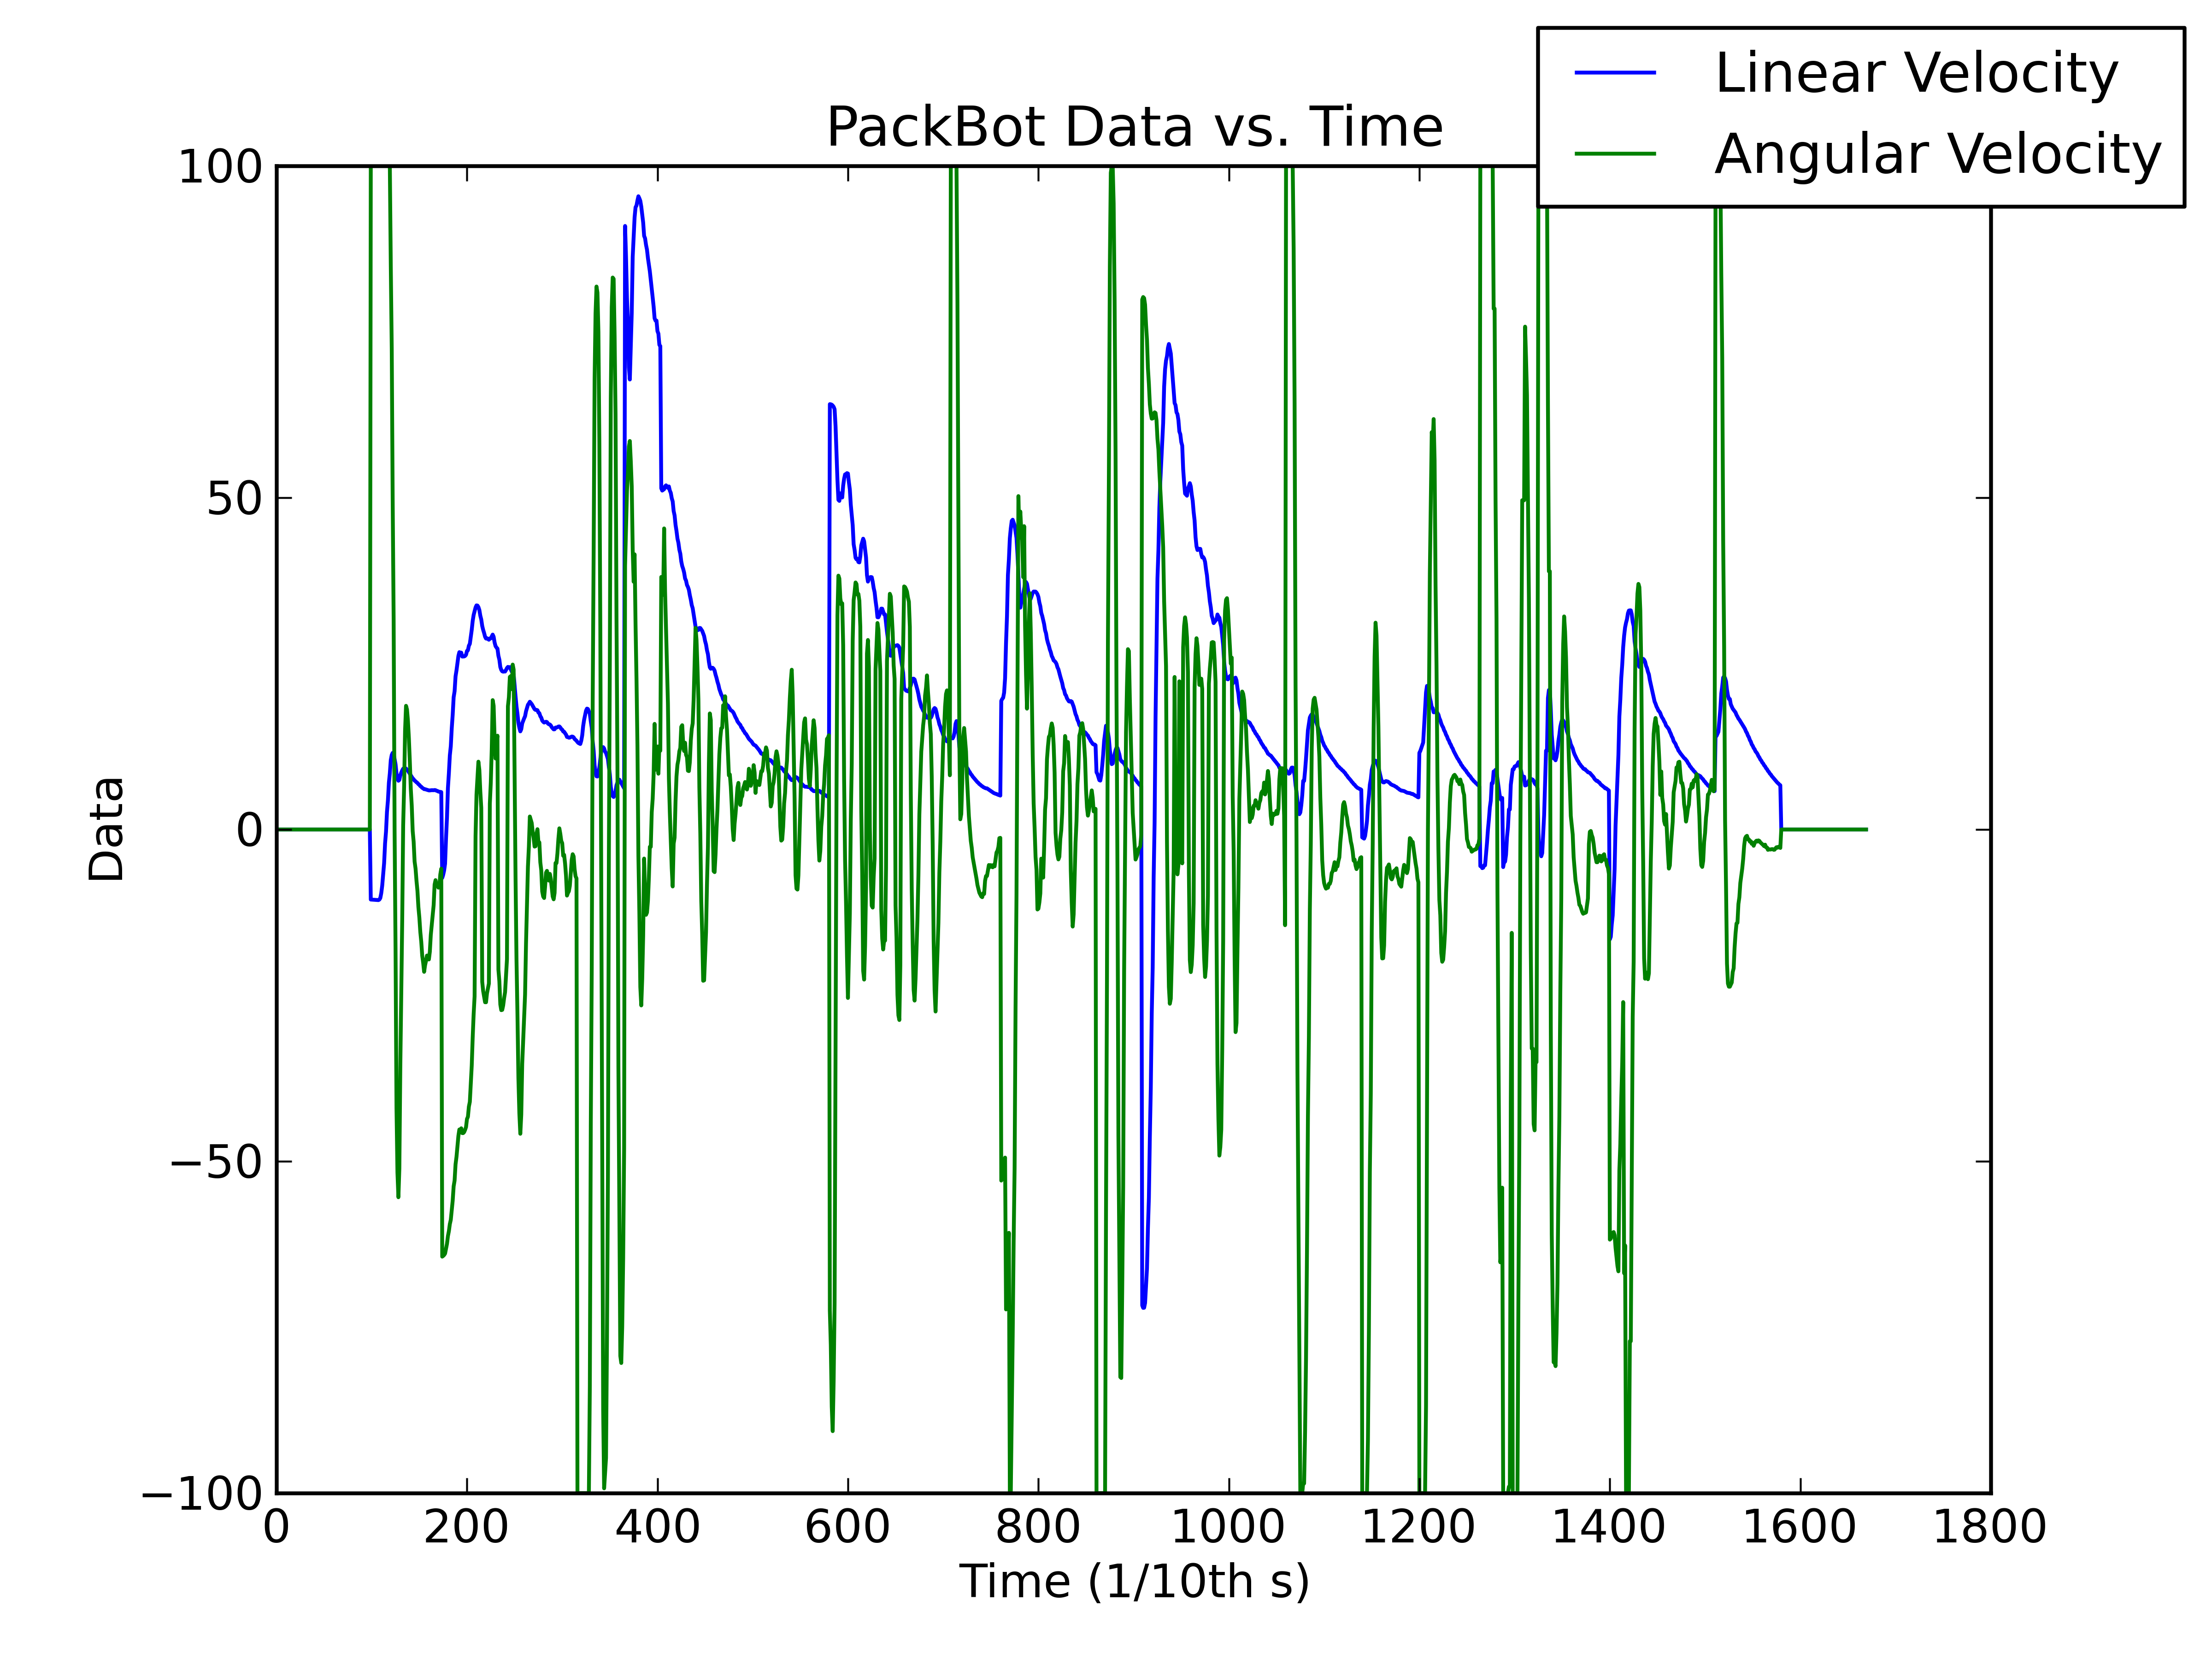
\includegraphics[width=.5\textwidth]{images/pbtx/20101203_1551_pbtxLyapOrigQR}
	\caption{Model Based Controller with Original Noise Models}
	\label{fig:resultsLyapunov1}
\end{figure}

\begin{figure}[ht!]
	\centering
	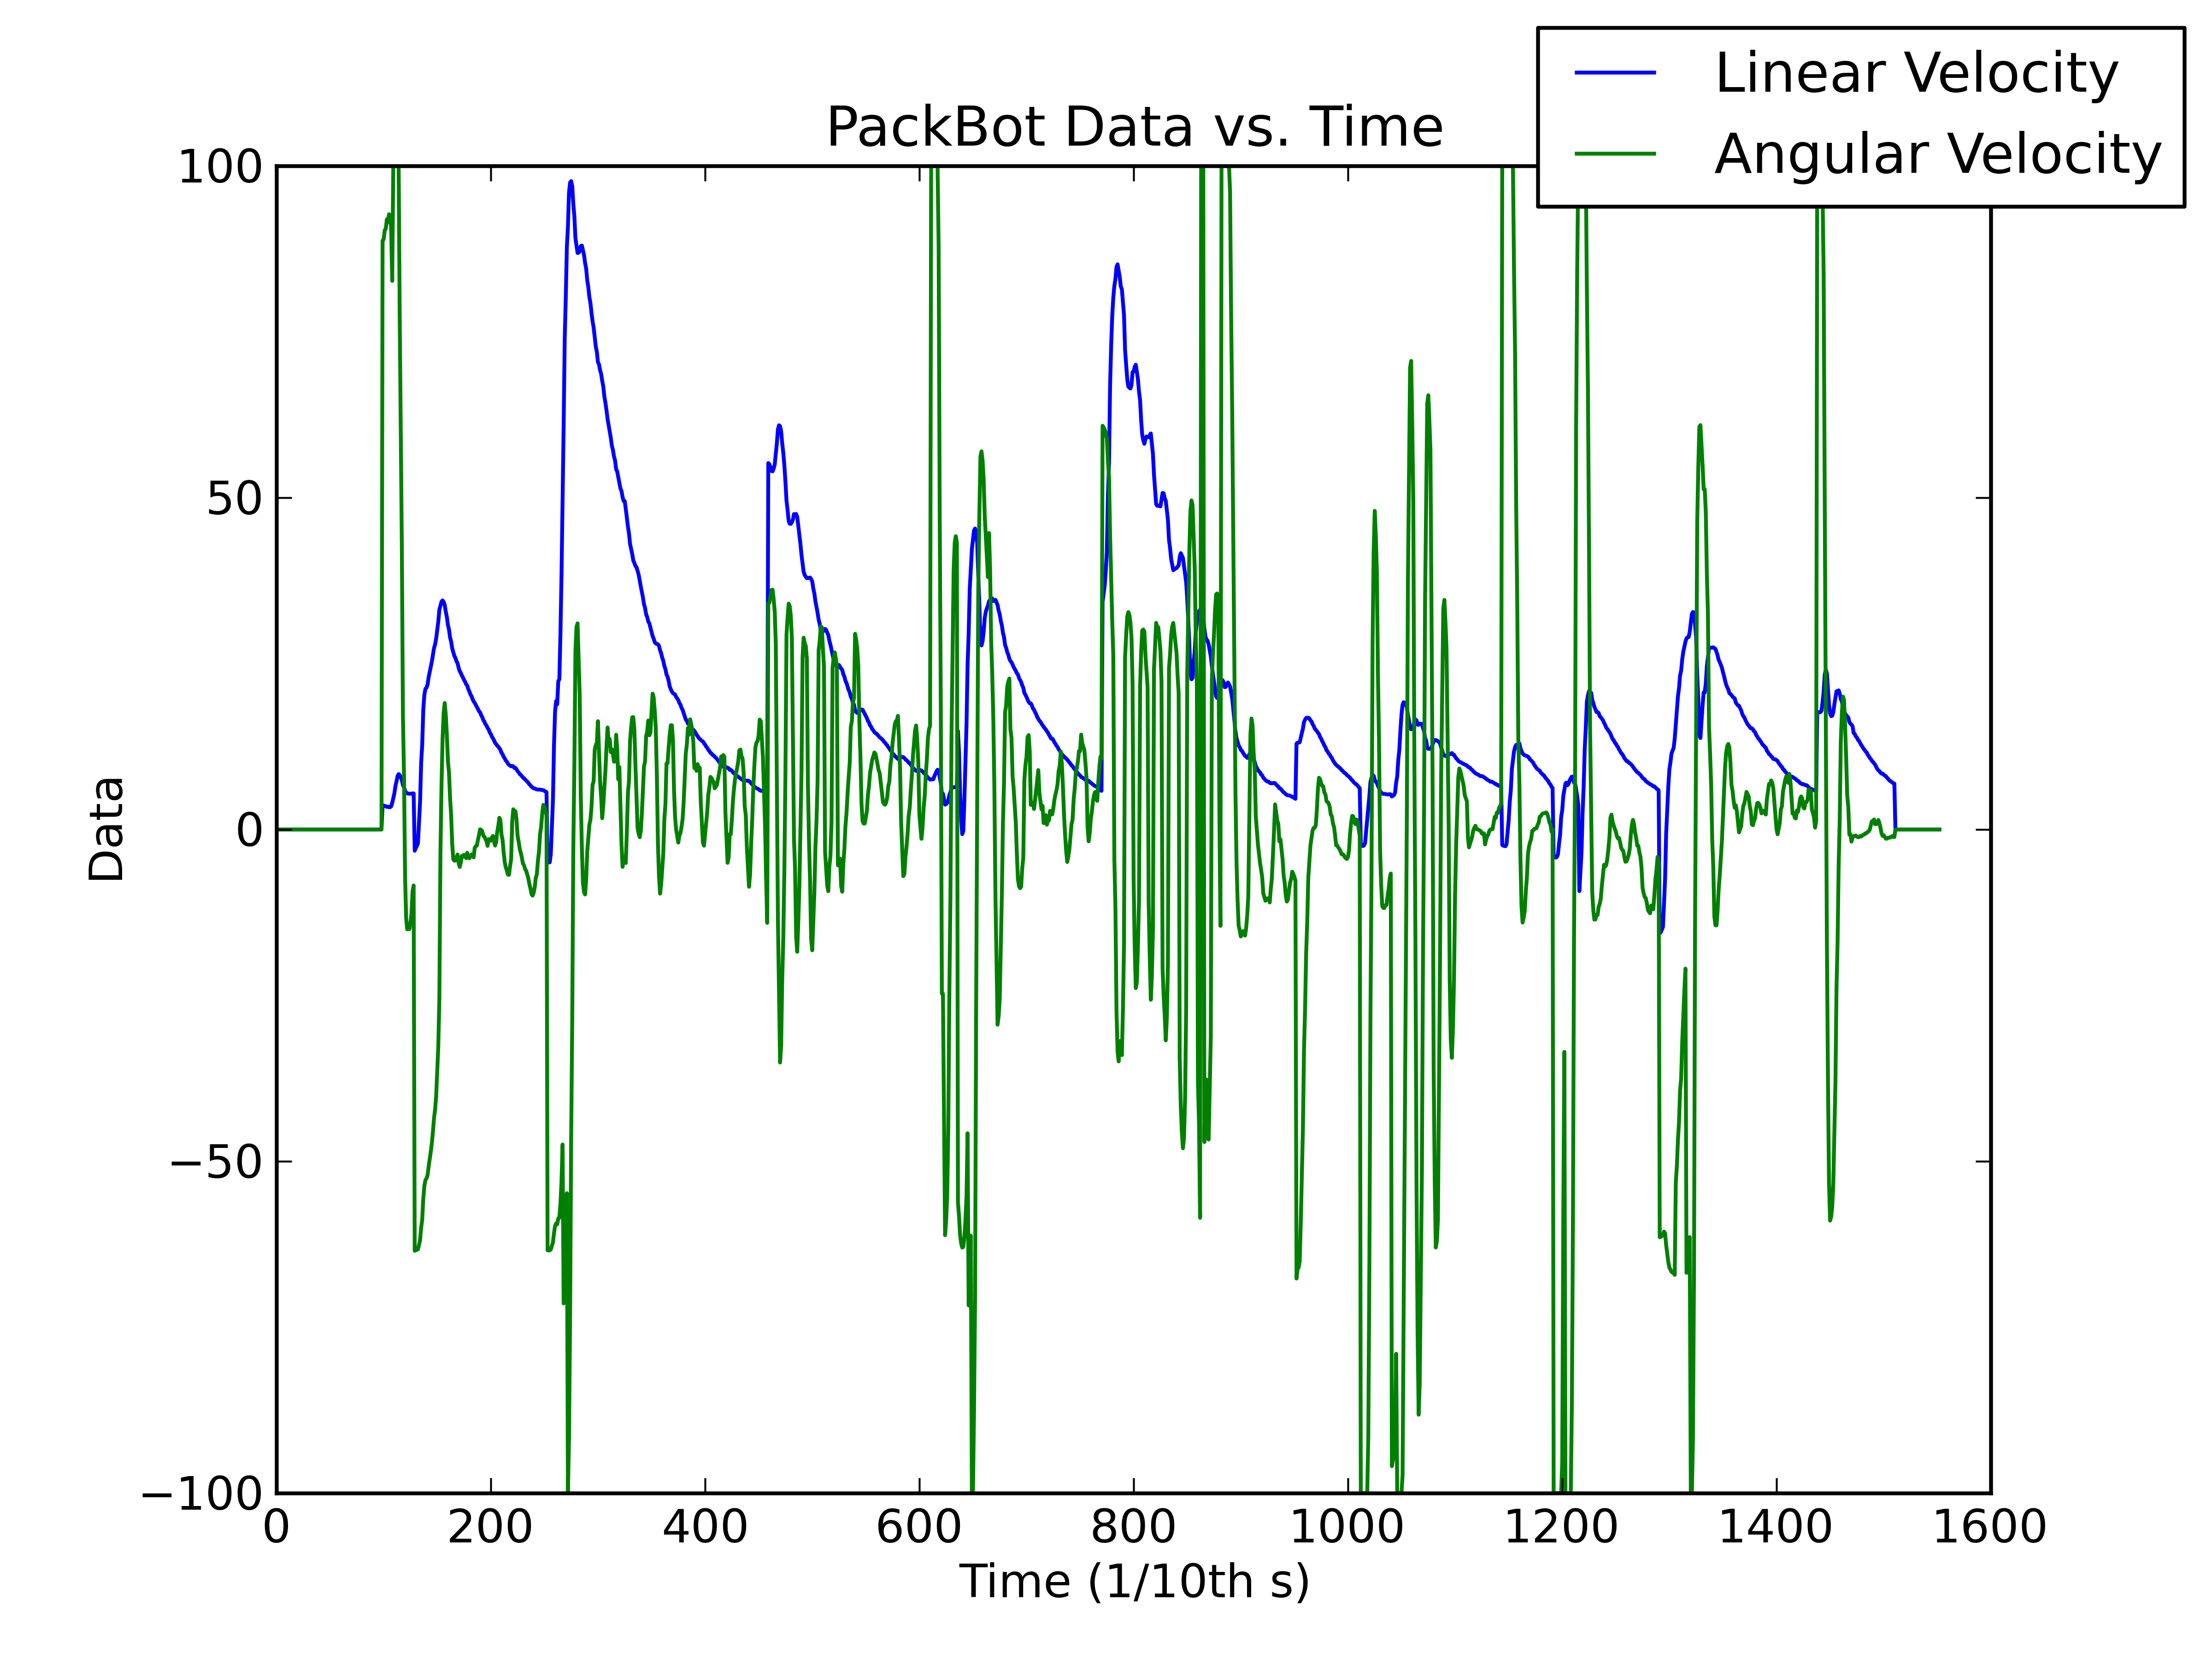
\includegraphics[width=.5\textwidth]{images/pbtx/20101203_1545_pbtxLyapNewQR}
	\caption{Model Based Controller with Learned Noise Models}
	\label{fig:resultsLyapunov2}
\end{figure}

\begin{figure}[ht!]
	\centering
	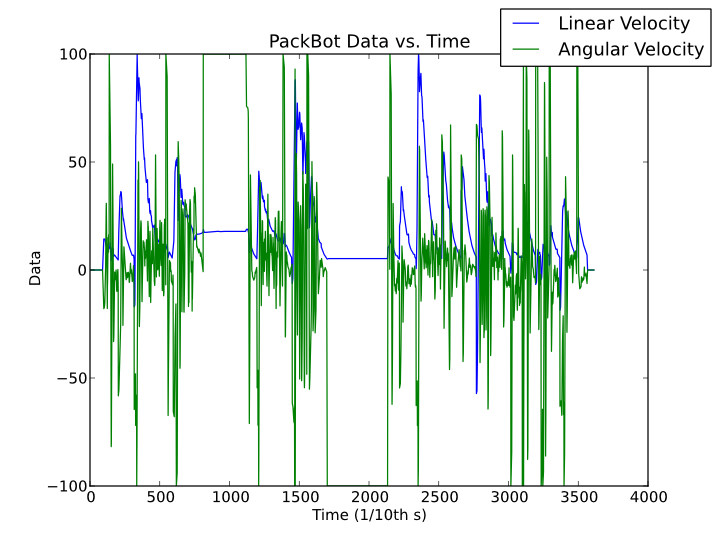
\includegraphics[width=.5\textwidth]{images/pbtx/20101203_1606_pbtxLyapUsingDgpsNewQR}
	\caption{Model Based Controller Using DGPS with Learned Noise Models}
	\label{fig:resultsLyapunov3}
\end{figure}

\begin{figure}[ht!]
	\centering
	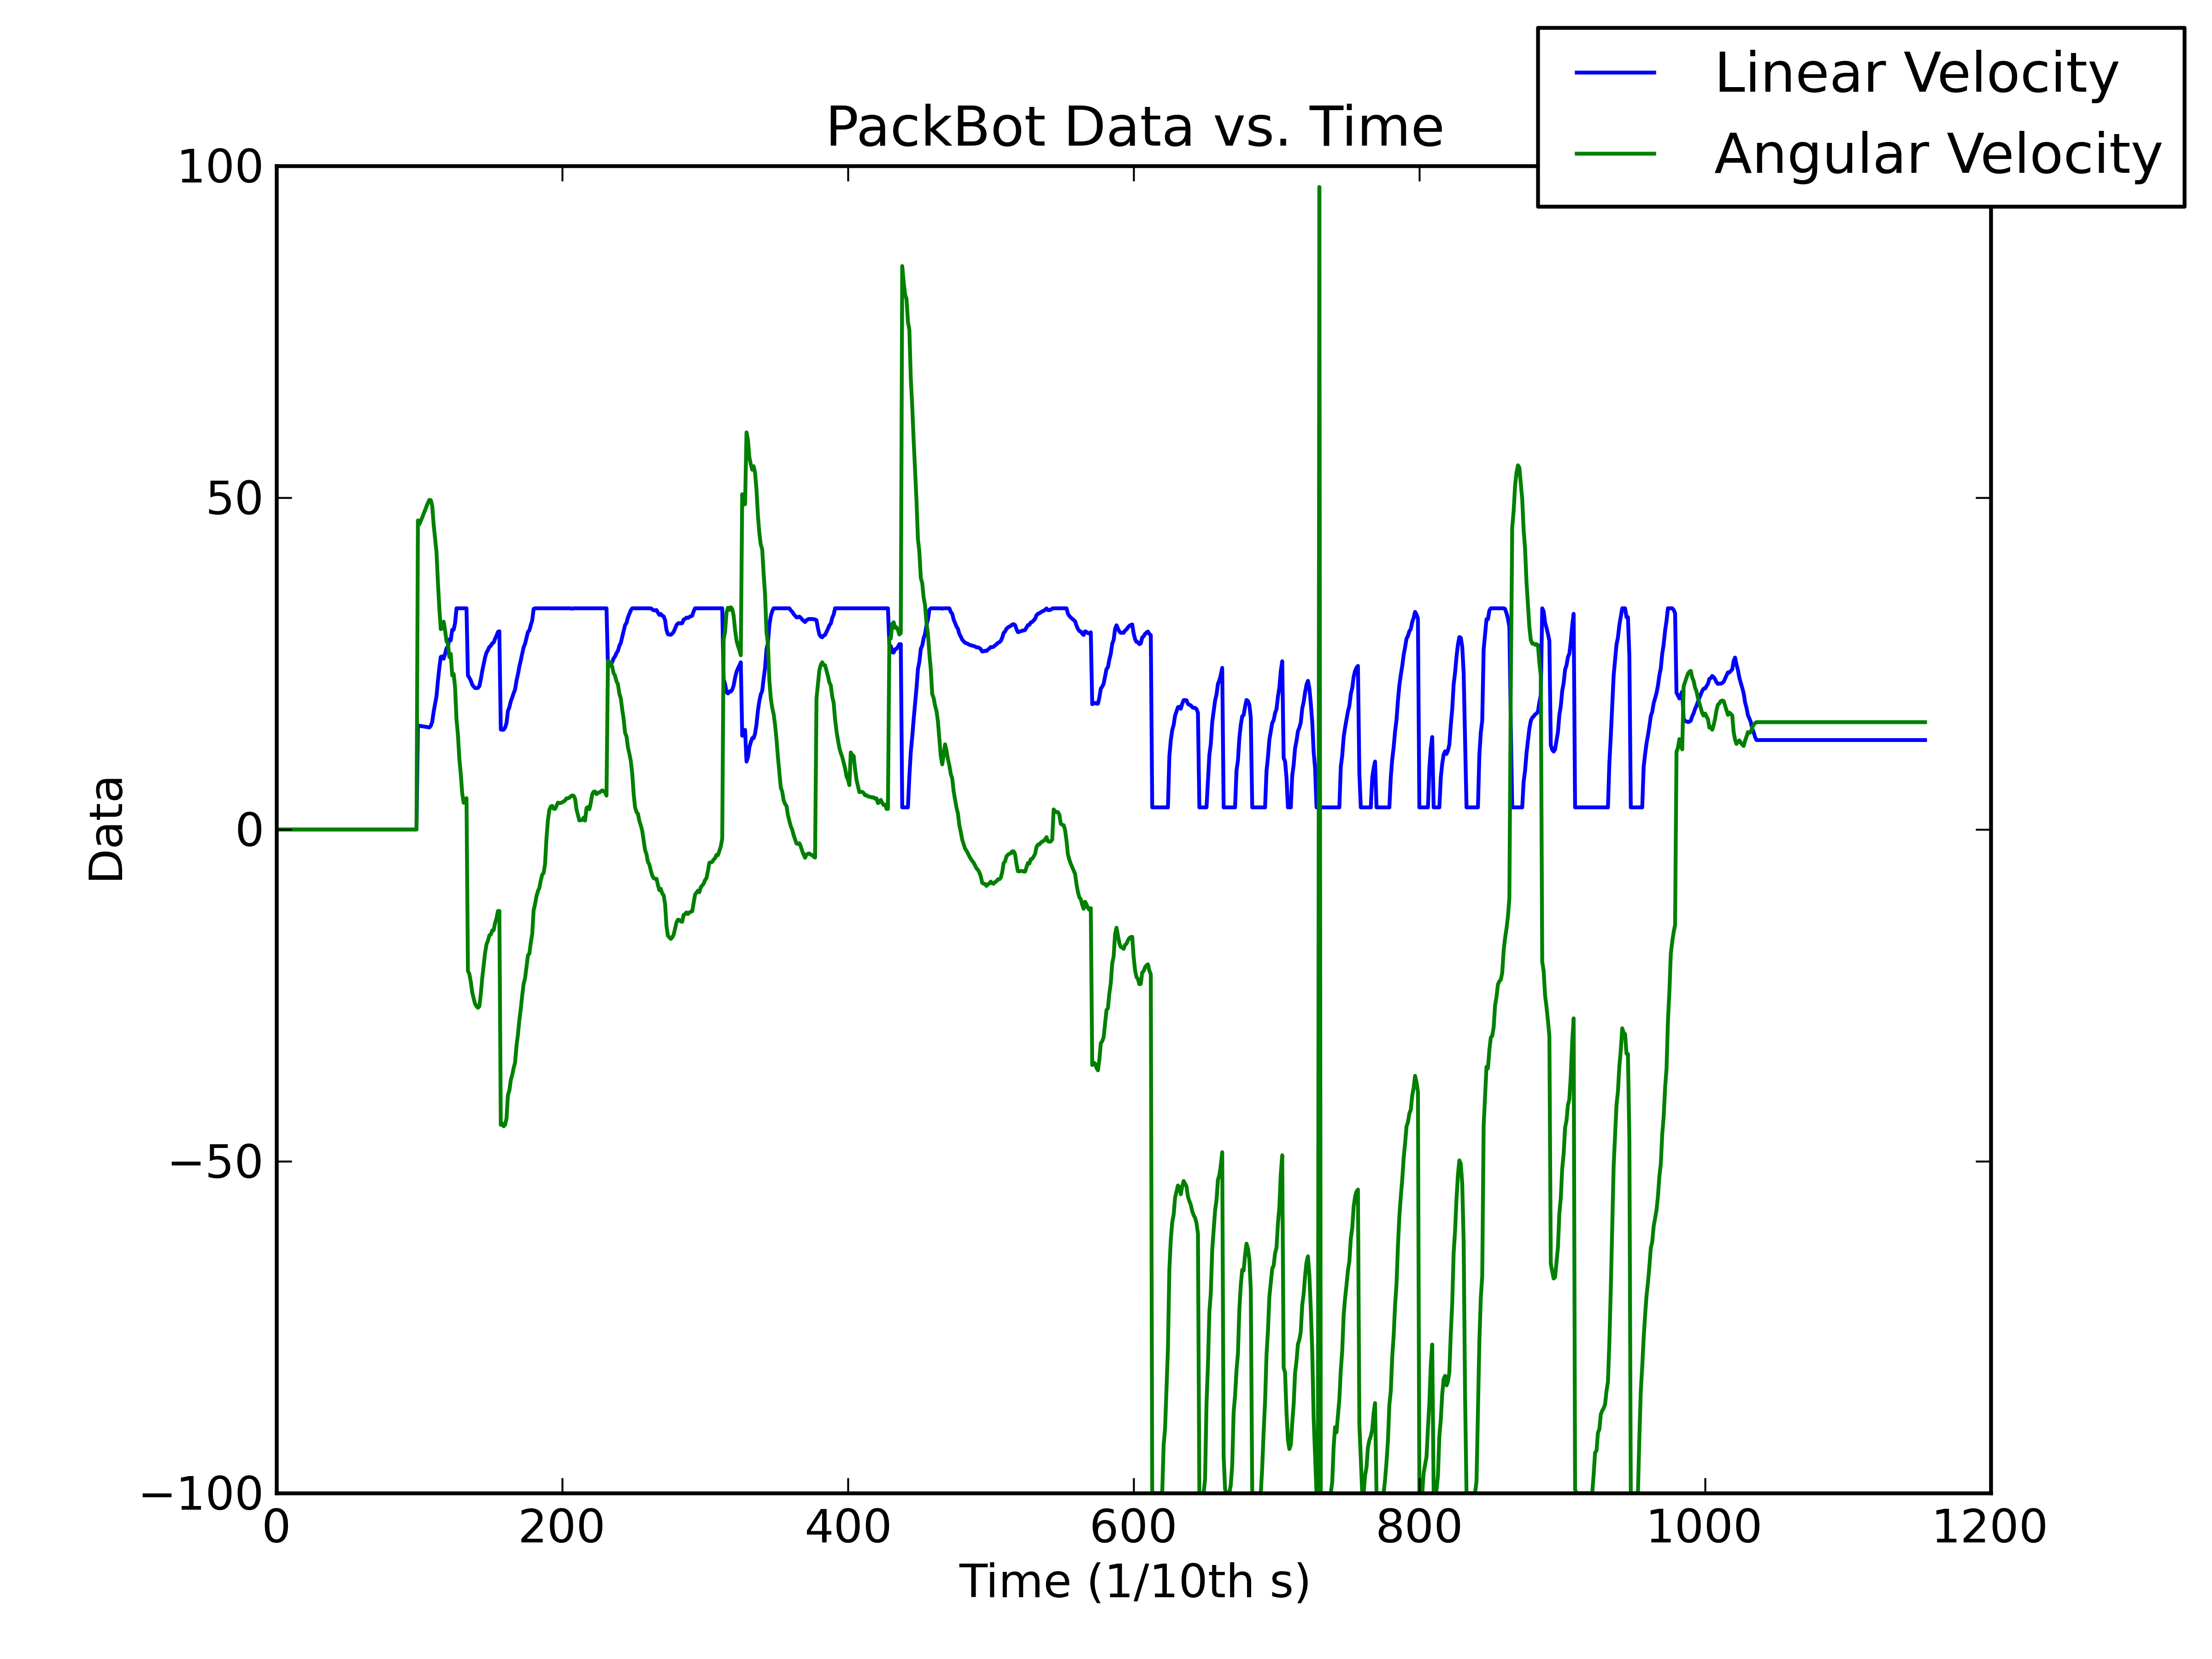
\includegraphics[width=.5\textwidth]{images/pbtx/20101203_1755_pbtxPidOrigQR}
	\caption{PID Controller with Original Noise Models}
	\label{fig:resultsLyapunov4}
\end{figure}

\begin{figure}[ht!]
	\centering
	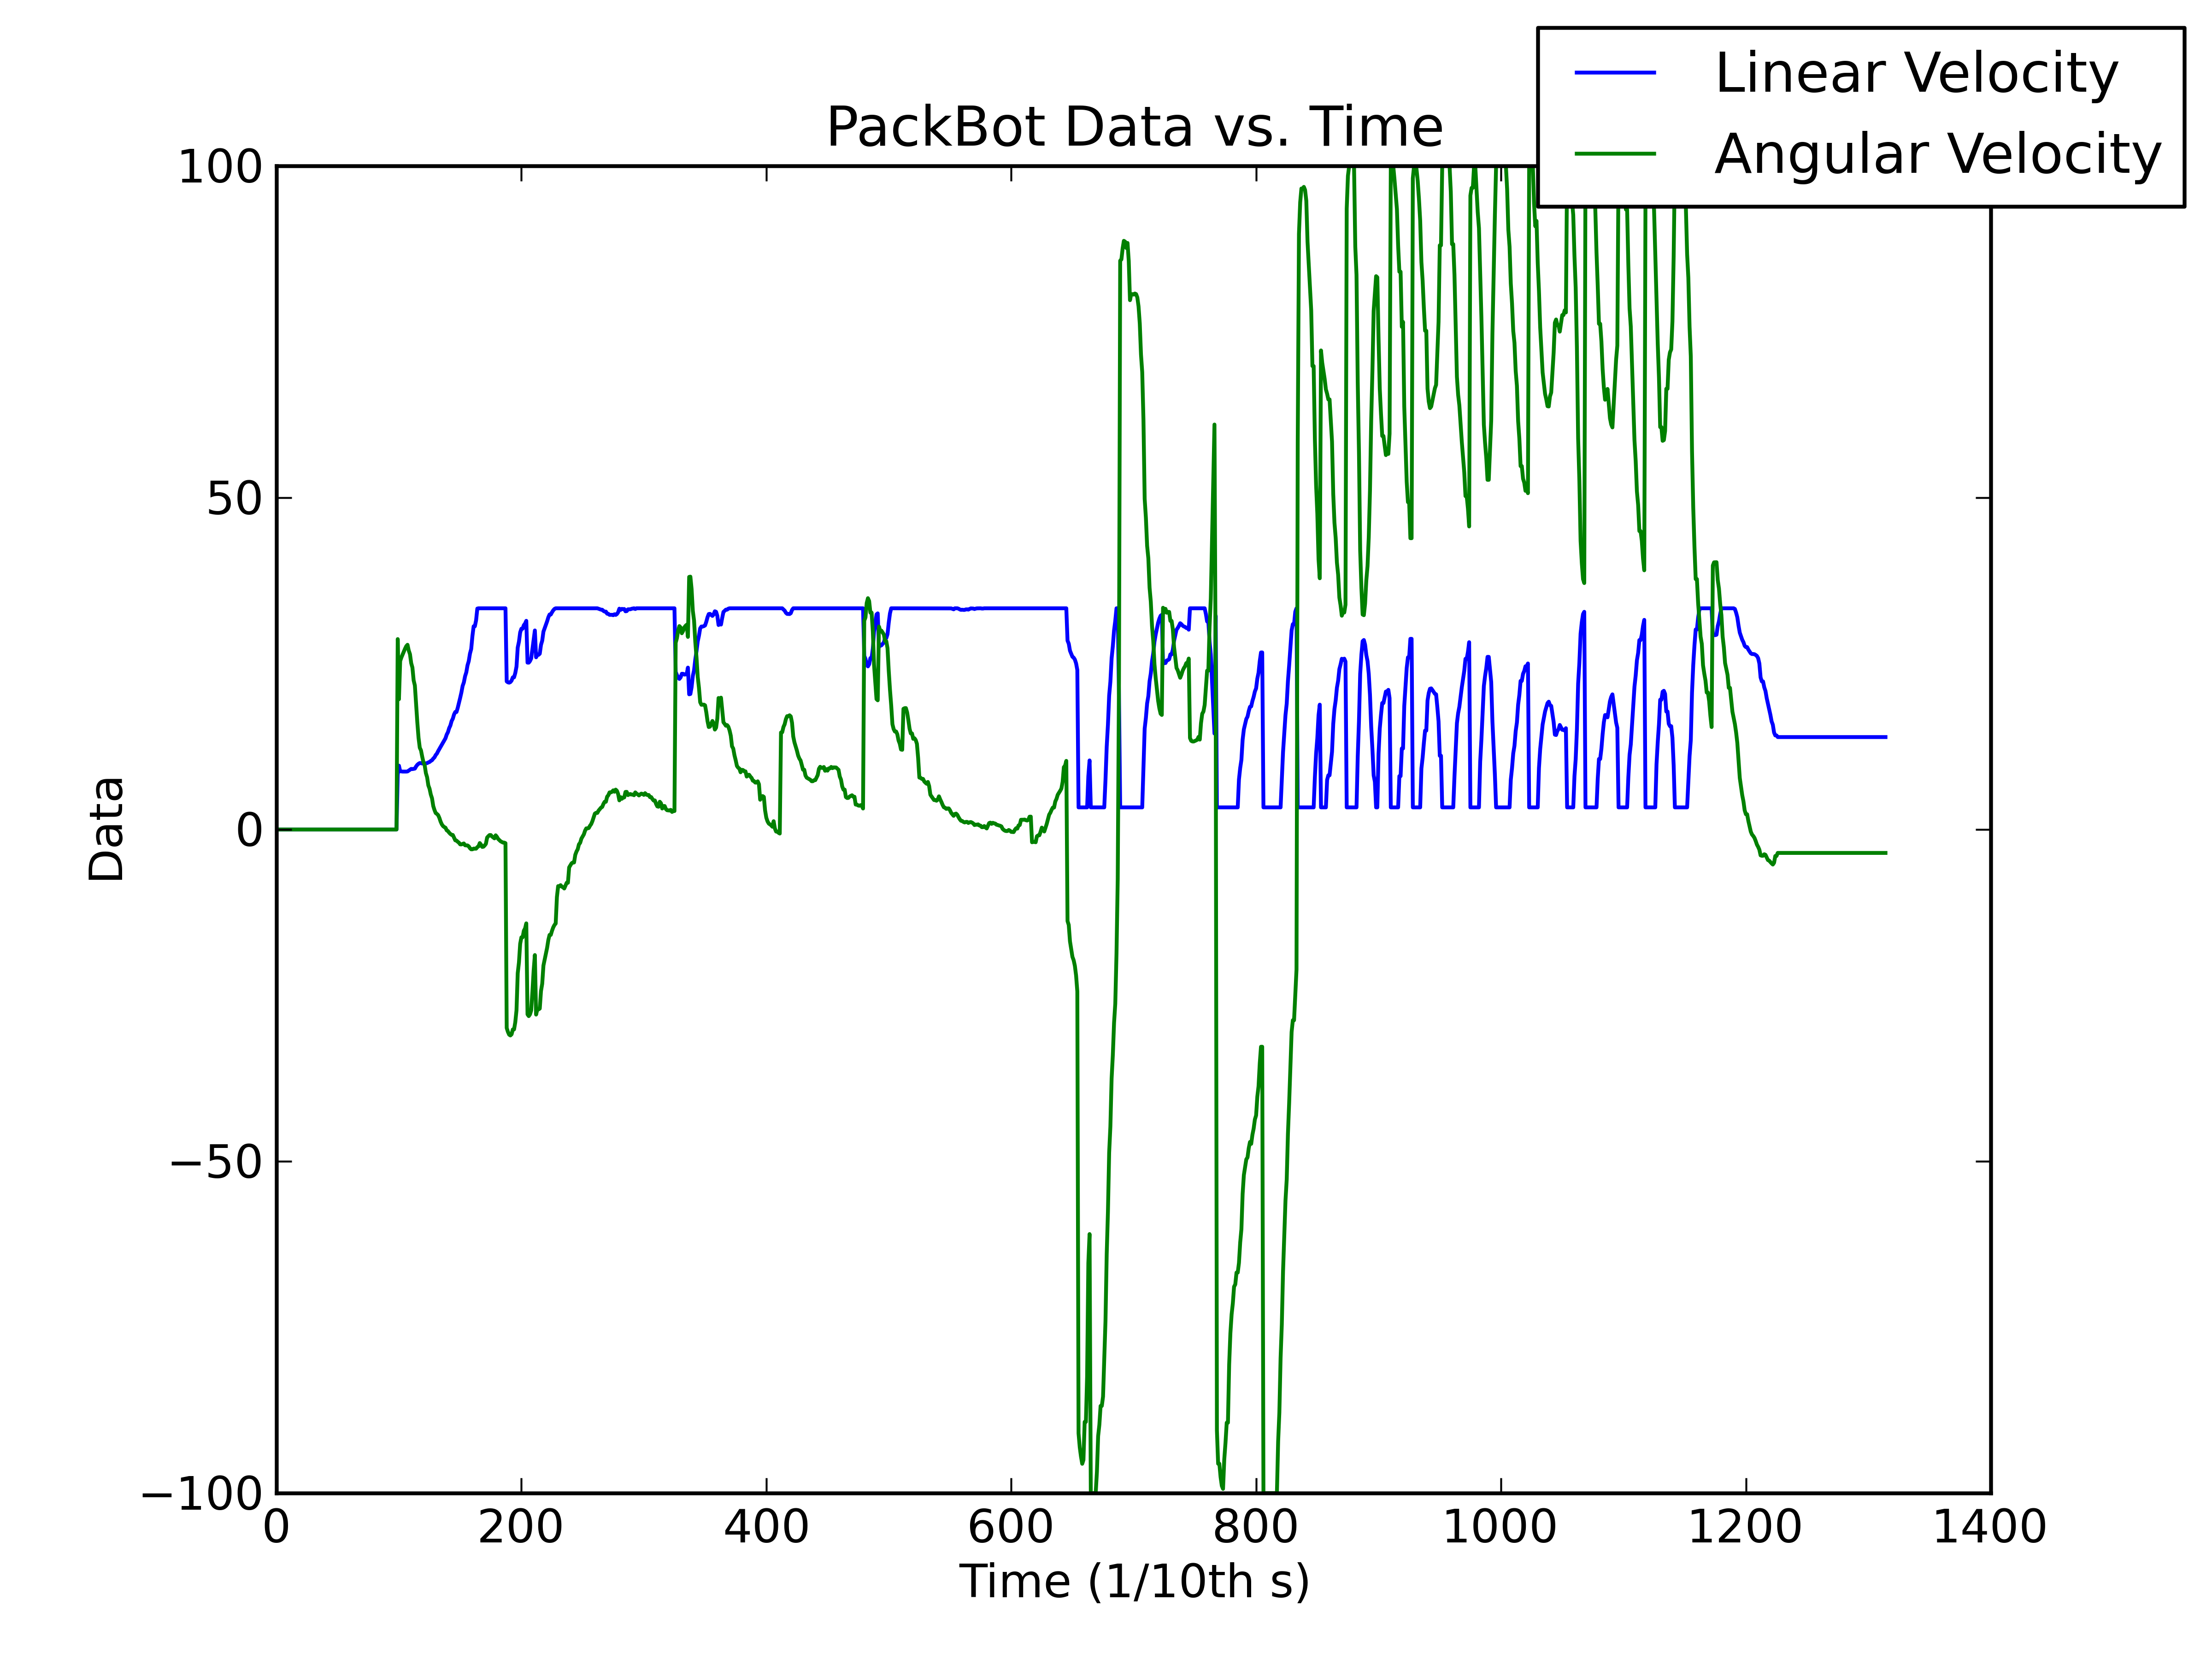
\includegraphics[width=.5\textwidth]{images/pbtx/20101203_1751_pbtxPidNewQR}
	\caption{PID Controller with Learned Noise Models}
	\label{fig:resultsLyapunov5}
\end{figure}

\begin{figure}[ht!]
	\centering
	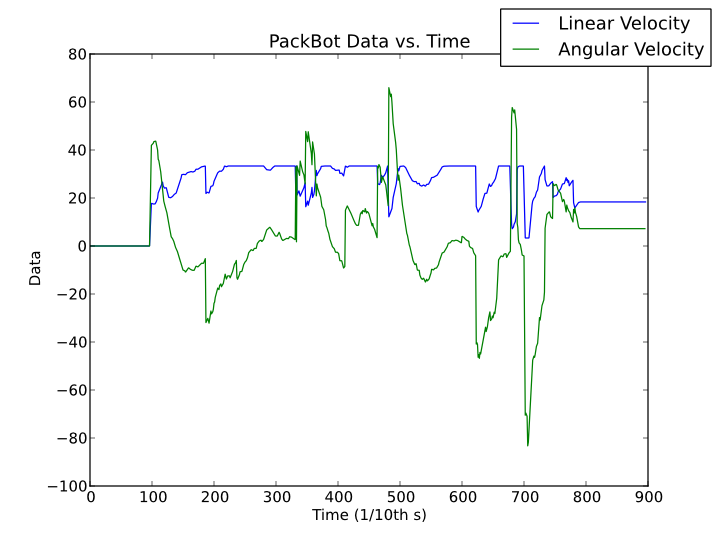
\includegraphics[width=.5\textwidth]{images/pbtx/20101203_1803_pbtxPidUsingDgpsNewQR}
	\caption{PID Controller Using DGPS with Learned Noise Models}
	\label{fig:resultsLyapunov6}
\end{figure}

The process of selecting gains in Chapter \ref{sec:lyapunovTrajectoryConvergence} only applies as $(\alpha, \theta)\to(0,0)$ but says nothing about what happens when the angle errors are not small. Empirically it was determined that the gains $h=0.25$, $k=0.2$ and $\gamma=0.2$ worked well in creating smooth trajectories and later it was found that these gains cause $\zeta=1$ so that, when the angle errors are small, the system $A$ is critically damped although $\sigma>\gamma$ so the distance error converges faster than the angle errors. The best results occurred when the gains were set to $h=0.25$, $k=0.2$ and $\gamma=0.2$ \textit{until} the angle errors were $|\alpha|<0.5$ \textit{and} $|\theta|<0.5$ radians which leads to the linear approximation being valid and the gains were then changed to $h=1.1$, $k=0.42$ and $\gamma=0.2$. This second set of gains, used when the angle errors were small, are critically damped for the system $A$ since $\zeta=1$ and the angle errors converge faster than the distance error since $\sigma>\gamma$. The results of this adaptive gain scheme can be seen in Figures \ref{fig:resultsLyapunovPositionAdaptive} and \ref{fig:resultsLyapunovVelocitiesAdaptive}. Note that the goal heading, $\theta^\star$, was set to be the angle from the current waypoint to the next waypoint so that the robot would be pointing in the direction of the next waypoint when it reached the current waypoint. For the last waypoint in the route the goal heading used was $\theta^\star=\alpha$.

\begin{figure}[ht!]
	\centering
	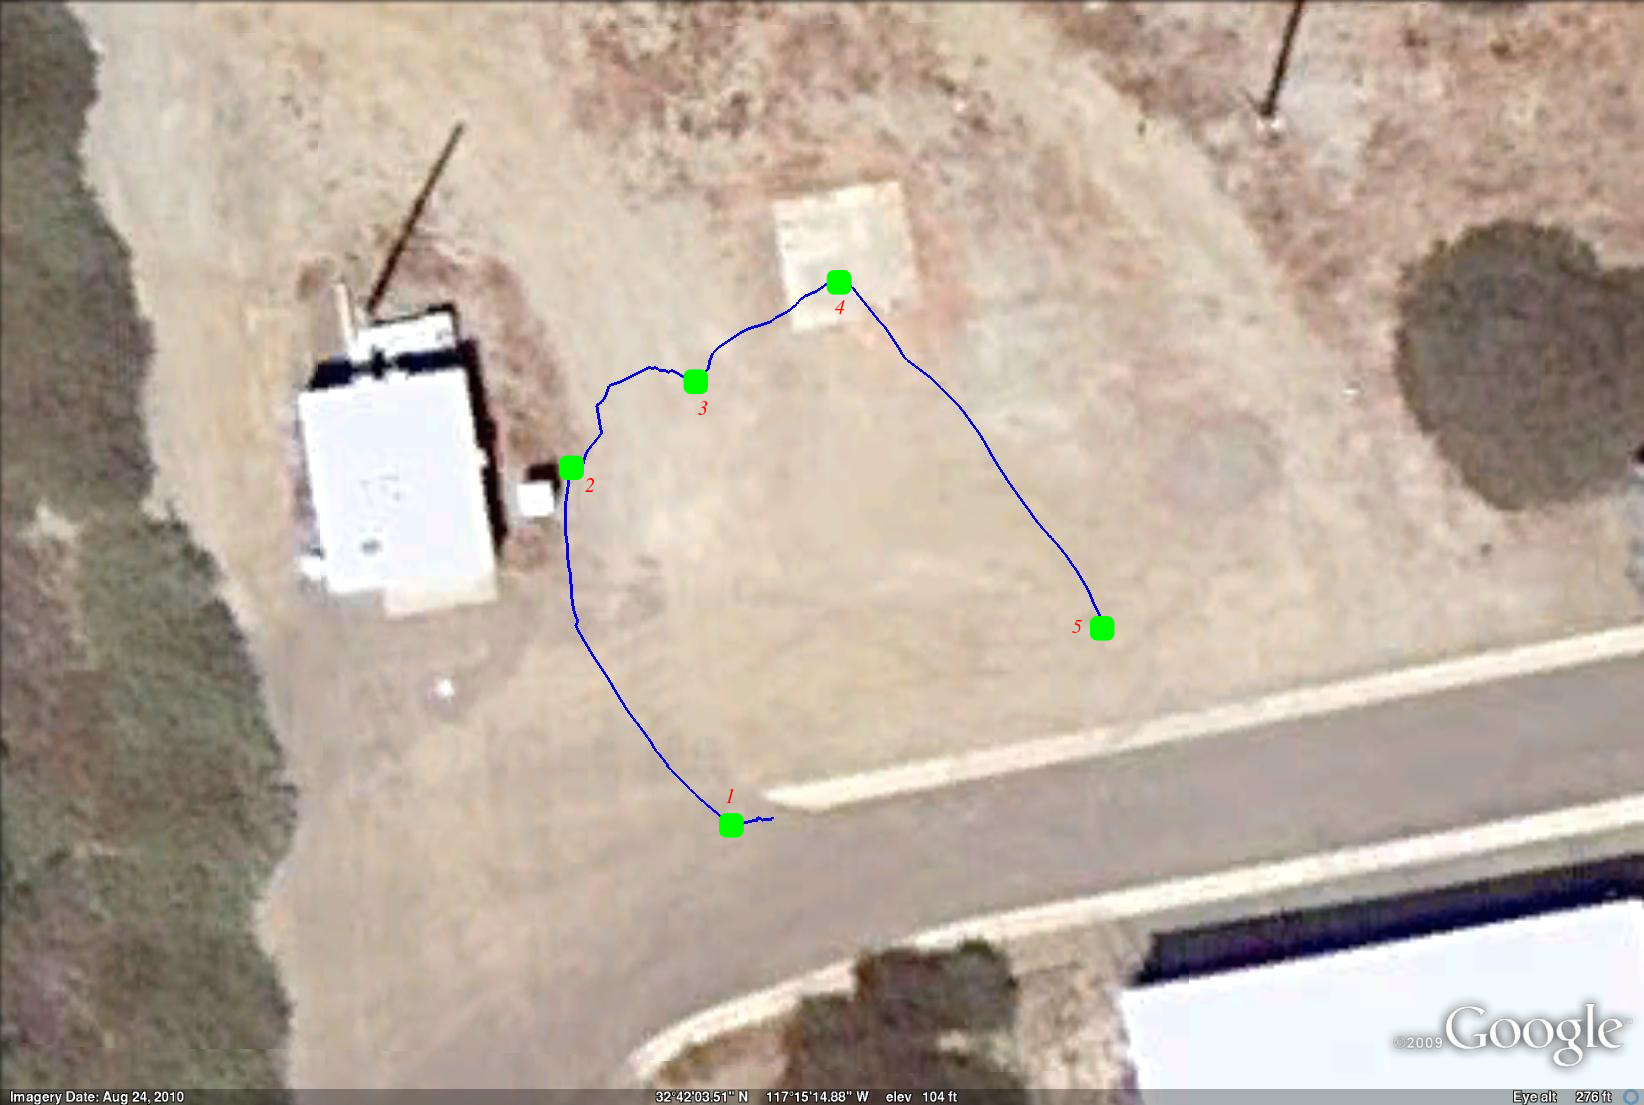
\includegraphics[width=.5\textwidth]{images/GE/20100929_1448_GE_KF_waypts}
	\caption{Robot Position using Adaptive Gain Scheme}
	\label{fig:resultsLyapunovPositionAdaptive}
\end{figure}

\begin{figure}[ht!]
	\centering
	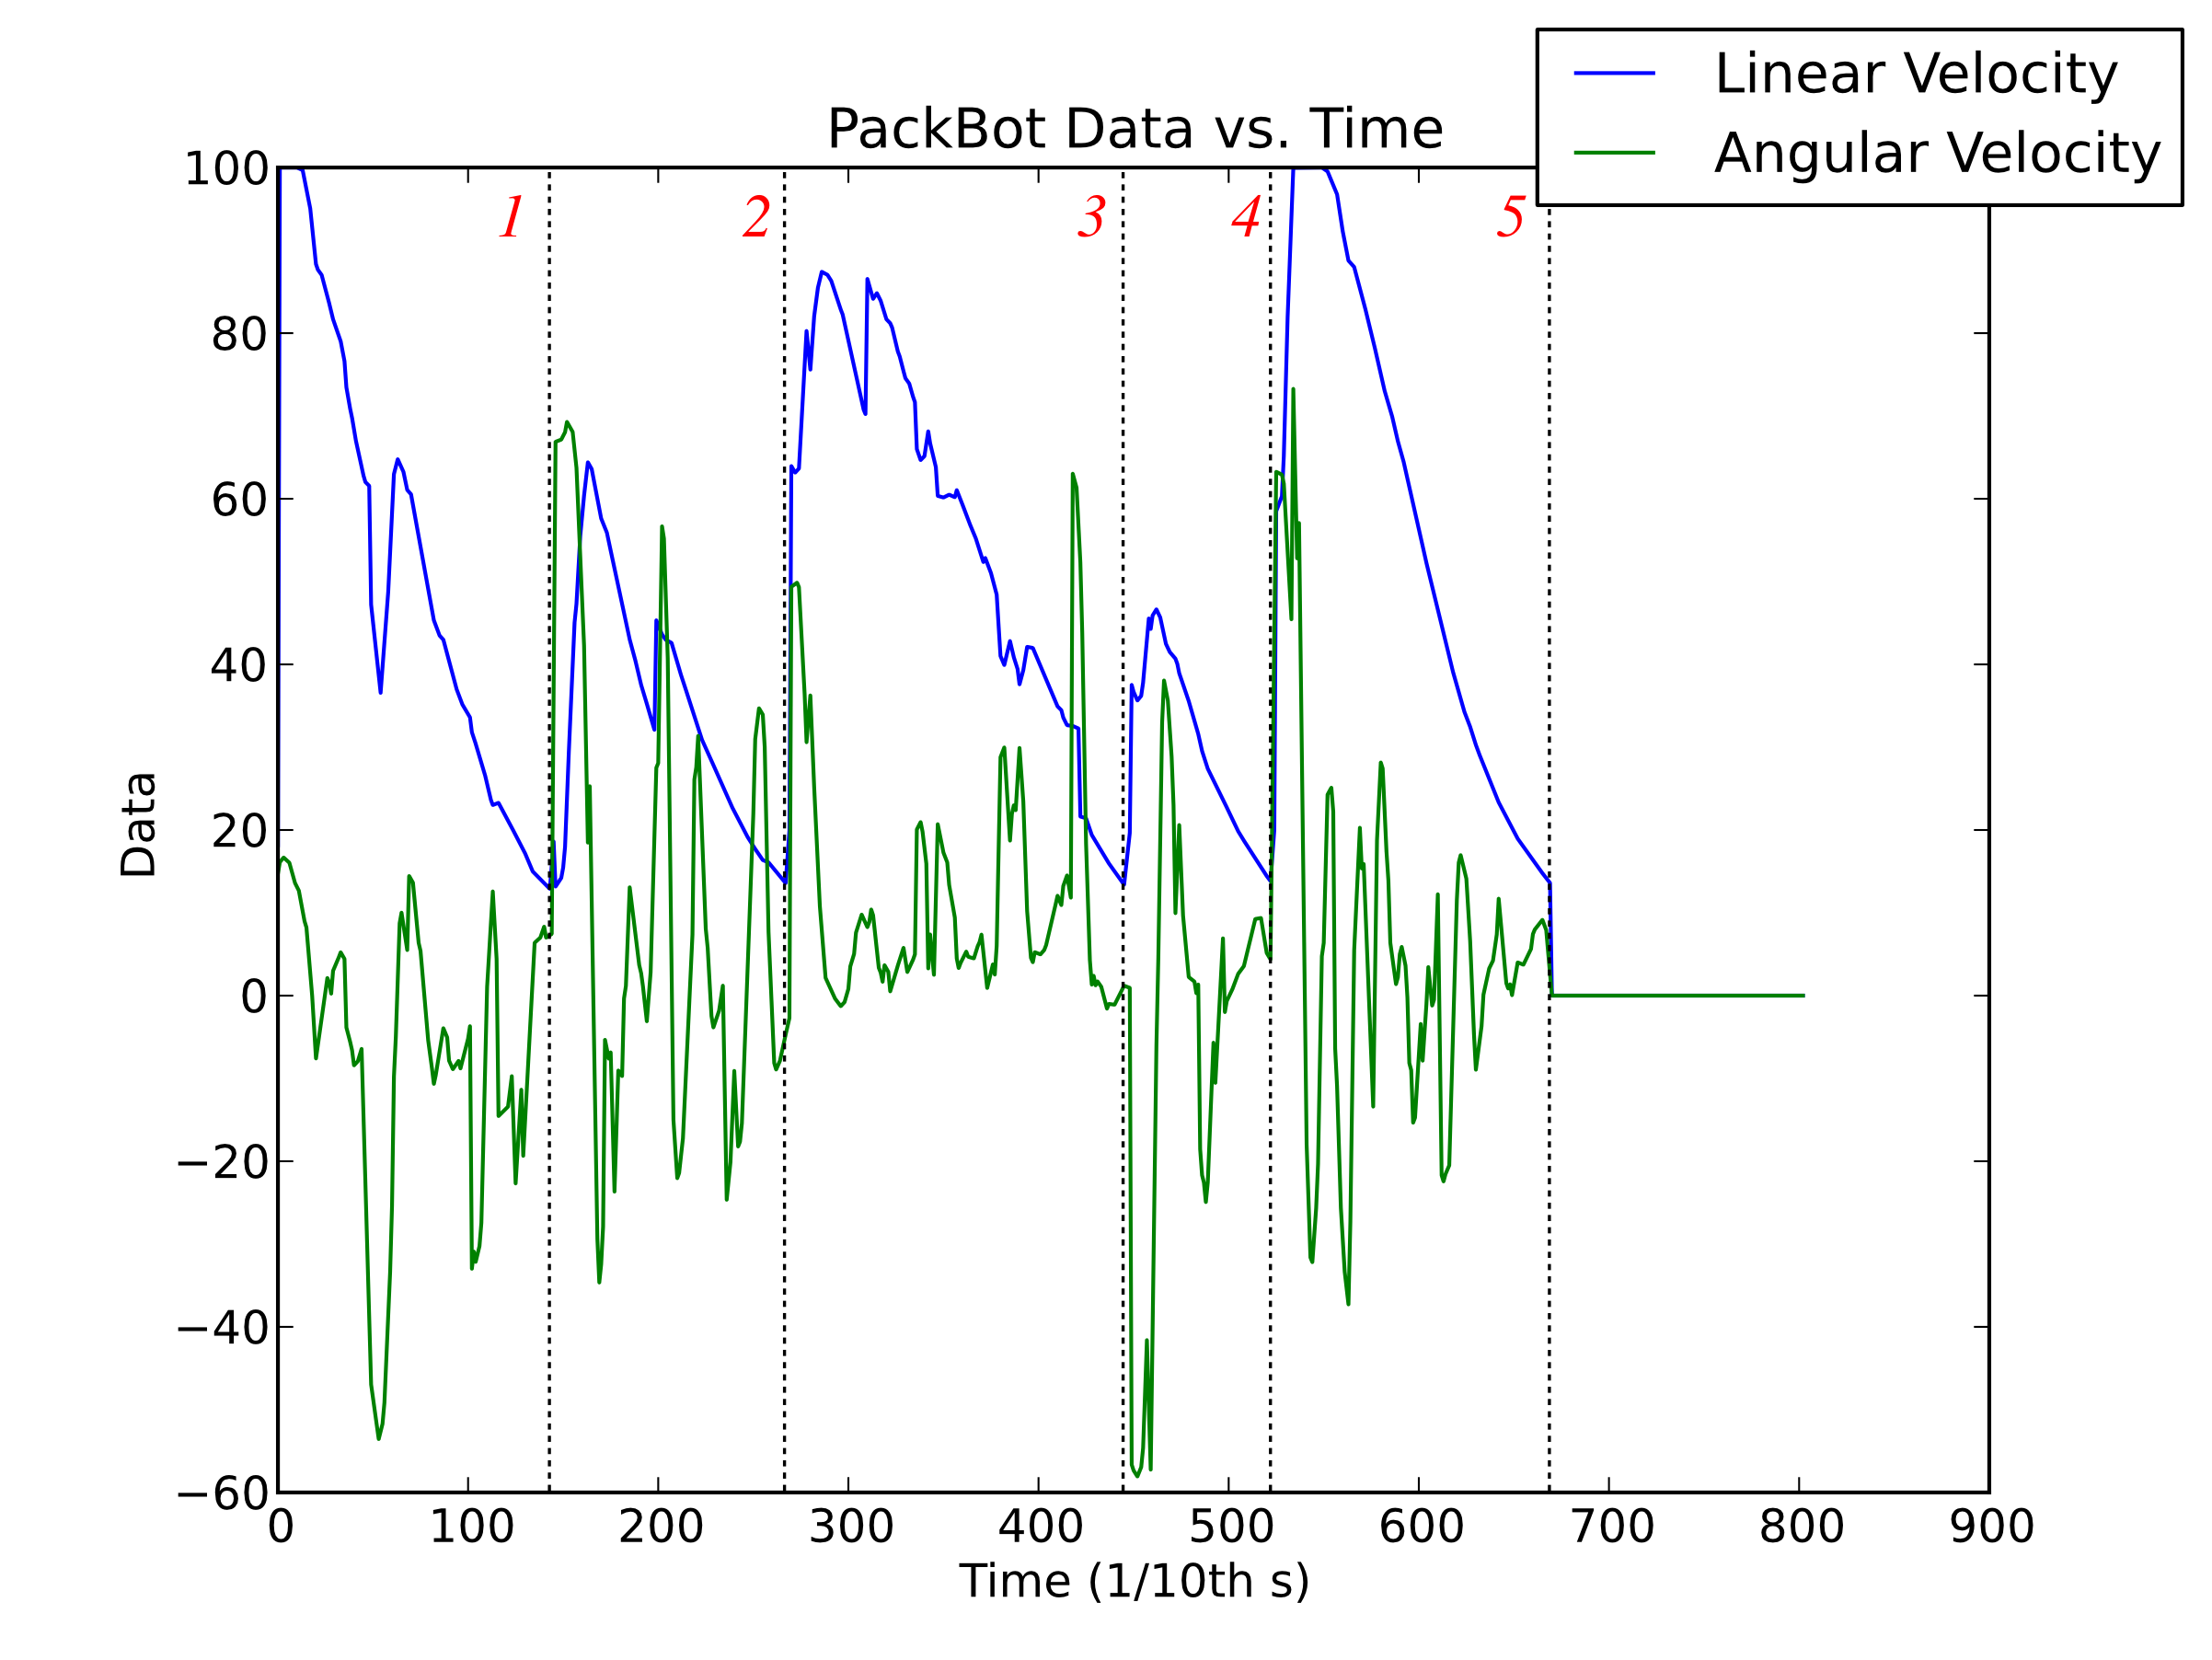
\includegraphics[width=.5\textwidth]{images/pbtx/20100929_1448_pbtx}
	\caption{Linear and Angular Velocities with Adaptive Gain Scheme}
	\label{fig:resultsLyapunovVelocitiesAdaptive}
\end{figure}

\subsection{Controller Comparison}
\label{sec:controllerComparison}
For both PID (Chapter \ref{sec:pid}, Table \ref{tab:PIDGainEffects}) and the model based controller (Chapter \ref{sec:lyapunovTrajectoryConvergence}) gains have to be selected, the difference being that stability is the goal when selecting PID gains whereas stability is guaranteed with the model based controller. More advanced behaviors such as three point turns are a consequence of the control law in (\ref{eq:lyapunovControlLaw}) derived using a kinematic model of the robot. The other very large difference between the controllers is that a table of gains must be tuned for the PID controller to work at varying linear velocities but the model based controller works very well at different linear and angular velocities. Also, when properties of the robot such as mass are changed by using different payloads for the system the entire table of PID gains must be retuned while, at most, one set of gains must be retuned for the model based controller. This last benefit of the model based controller makes it very appealing to use in fielded systems since it reduces the amount of maintenance and effort required to keep the robot in working condition. The model based controller will also allow for improved navigation performance near obstacles which leads directly to improved autonomy for the robot.

Many different controller configurations are possible based on varying the gains used and the calculation of the desired heading at waypoints. The tested configurations included:
\begin{enumerate}
\item PID with best available gains,
\item Fuzzy logic with best available rules,
\item Model based with $\theta^\star$ set as angle from current waypoint to next waypoint with gains set to minimize distance error before angle errors ($\gamma = $, $h = $, $k = $),
\item Model based with $\theta^\star$ set as angle from previous waypoint to current waypoint with gains set to minimize distance error before angle errors ($\gamma = $, $h = $, $k = $),
\item Model based with $\theta^\star$ set as average of angles from previous waypoint to current waypoint and from current waypoint to next waypoint with gains set to minimize distance error before angle errors ($\gamma = $, $h = $, $k = $),
\item Model based with $\theta^\star$ set as angle from current waypoint to next waypoint with gains set to minimize angle errors before distance error ($\gamma = $, $h = $, $k = $),
\item Model based with $\theta^\star$ set as angle from previous waypoint to current waypoint with gains set to minimize angle errors before distance error ($\gamma = $, $h = $, $k = $),
\item Model based with $\theta^\star$ set as average of angles from previous waypoint to current waypoint and from current waypoint to next waypoint with gains set to minimize angle errors before distance error ($\gamma = $, $h = $, $k = $),
\item Model based with $\theta^\star$ set as angle from current waypoint to next waypoint with gains set to minimize distance error before $\alpha$ before $\theta$ ($\gamma = $, $h = $, $k = $),
\item Model based with $\theta^\star$ set as angle from previous waypoint to current waypoint with gains set to minimize distance error before $\alpha$ before $\theta$ ($\gamma = $, $h = $, $k = $),
\item Model based with $\theta^\star$ set as average of angles from previous waypoint to current waypoint and from current waypoint to next waypoint with gains set to minimize distance error before $\alpha$ before $\theta$ ($\gamma = $, $h = $, $k = $),
\item Model based with parking behavior turned on and gains ($\gamma = $, $h = $, $k = $).
\end{enumerate}
Note that in all cases for the model based controller the desired goal heading $\theta^\star$ for the final waypoint was set to be the angle from the previous waypoint to the last waypoint.

Each controller configuration was run on several courses that test specific behaviors such as allowing for maximum velocities to be sustained with large amounts of open space on the route by having long path segments, short path segments between waypoints to simulate obstacles along the route and a mixture of long and short path segments.

The results using the different setups described are shown in Table \ref{tab:resultsControllers} where the metrics used to compare the controller performance are
\begin{itemize}
\item the time required to complete the course,
\item the average cross track error during the course to show whether the robot followed a straight line between waypoints which is important when obstacles are in the area and not important when large amounts of open space are available for navigation (although some operators become nervous when the robot trajectory has large curvature even if open space is available),
\item the maximum velocity achieved by the robot during the course,
\item the number of times that the robot stops where a stop is defined as the robot having a velocity that drops below a small velocity.
\end{itemize}

\begin{table}[ht!]
\caption{Controller Comparison}
\small
\centering
\begin{tabular}{@{}llllr@{}} \toprule
Setup & Time (s) & Cross Track Error (m) & Max Velocity (m/s) & \# Stops \\ \midrule
1     & 0        & 0                     & 0                  & 0        \\
2     & 0        & 0                     & 0                  & 0        \\
3     & 0        & 0                     & 0                  & 0        \\
4     & 0        & 0                     & 0                  & 0        \\
5     & 0        & 0                     & 0                  & 0        \\
6     & 0        & 0                     & 0                  & 0        \\
7     & 0        & 0                     & 0                  & 0        \\
8     & 0        & 0                     & 0                  & 0        \\
9     & 0        & 0                     & 0                  & 0        \\
10    & 0        & 0                     & 0                  & 0        \\
11    & 0        & 0                     & 0                  & 0        \\
12    & 0        & 0                     & 0                  & 0        \\ \bottomrule
\end{tabular}
\label{tab:resultsControllers}
\end{table}
